\documentclass{beamer}
\usepackage{tikz}
\usepackage{pgfplots}
\usepackage{multicol}

\title{Ruído em Sistemas AM e FM}
\subtitle{Princípios de Comunicação para Engenharia }
\author{Prof. Daniel C. Araújo}
\institute{Universidade de Brasília}
\date{\today}

\begin{document}

\frame{\titlepage}


\section{Exercícios}


\begin{frame}
  \frametitle{Exercício 1}

  \begin{block}{Questão}
    O sinal recebido $r(t) = s(t) + n(t)$ em um sistema de Comunicação
    passa por um filtro passa-baixa de largura de banda $W$ e ganho unitário.
    A componente $s(t)$ possui densidade espectral de potência
    $$
    S_s(f) = \frac{P_0}{1+\left(\frac{f}{B}\right)^2},
    $$
    em que $B$ é a banda de 3 dB. A componente de ruído possui densidade
    espectral de potência $\frac{N_0}{2}$ $\forall f$ $\in$ $\mathbb{R}$. Determine e 
    e faça o gráfico da SNR como uma função de $W/B$. Qual a largura de banda $W$ que 
    resultará na máxima $SNR$.
  \end{block}

\end{frame}

\begin{frame}
  \frametitle{Solução}

    O espectro do sinal na saída do filtro é
    $S_o(f) = S_s(f) |\Pi \left(\frac{f}{2W}\right)|^2$. Portanto, 
    a potência do sinal é 
    
    Se $W/B > 0$, a solução é:
    \begin{align*}
    \int_{-W}^{W} \frac{P_0}{1 + \left(\frac{f}{B}\right)^2} df &= P_0 B \left[\arctan\left(\frac{f}{B}\right)\right]_{-W}^{W} \\
    &= P_0 B \left(\arctan\left(\frac{W}{B}\right) - \arctan\left(-\frac{W}{B}\right)\right) \\
    &= P_0 B \cdot 2 \arctan\left(\frac{W}{B}\right)
    \end{align*}

    A potência do ruído na saída do filtor é

    $$
    P_{n,o} = \int _{-W}^{W} \frac{N_0}{2}df = N_0 W
     $$

\end{frame}


\begin{frame}
  \frametitle{Solução}

  \begin{columns}
    \column{0.35\textwidth}
    \begin{align*}
      \text{SNR} &= \frac{P_0 B \cdot 2 \arctan\left(\frac{W}{B}\right)}{N_0 W} \\
      &= \frac{2P_0}{N_0} \frac{\arctan\left(\frac{W}{B}\right)}{\frac{W}{B}}
    \end{align*}
    \column{0.45\textwidth}
    \begin{figure}
      \centering 
  
      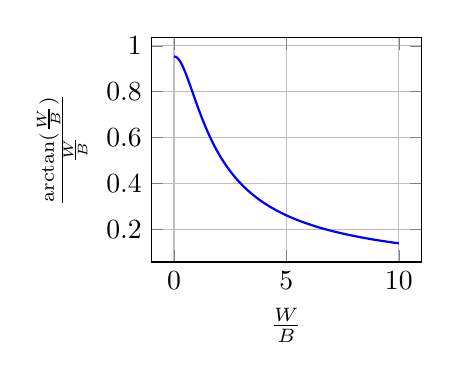
\begin{tikzpicture}
        \begin{axis}[
        domain=0.0001:10,
        xlabel=$\frac{W}{B}$,
        ylabel=$\frac{\arctan(\frac{W}{B})}{\frac{W}{B}}$,
        samples=100,
        smooth,
        scale=0.5,
        grid
        ]
        \addplot[blue,thick] {1/60*atan(x)/x};
        \end{axis}
      \end{tikzpicture}
  
  
    \end{figure}
    \end{columns}    
\end{frame}


\begin{frame}
  \frametitle{Questão 2}

  \begin{block}{Questão}
    Em um sistema de comunicação de radiodifusão, a 
    potência do transmissor é de 40 kW, a atenuação do canal é de 80 dB e a
     potência de ruído é de 4 x $10^{-10}$ W/Hz.

     \begin{itemize}
      \item Encontre o SNR pré-detecção (SNR em $r(t) = \alpha u(t) + n(t)$).
      \item Encontre o SNR de saída se a modulação for DSB.
      \item Encontre o SNR de saída se a modulação for SSB.
      \item Encontre o SNR de saída se a modulação for AM convencional com um índice de modulação de 0,85 e possuir uma potência normalizada de mensagem de 0,2.
      \end{itemize}
  \end{block}

\end{frame}

\begin{frame}
  \frametitle{Solução}

  \begin{itemize}
    \item  Como a atenuação do canal é de 80 dB, então: 
    \begin{align*}
      P_R &= 10^{-8} \cdot P_T \\
        &= 10^{-8} \cdot 40 \cdot 10^3 \\
        & = 4 \cdot 10^{-4} \text{ Watts}
      \end{align*}
      Se o filtro limitador de ruído tem largura de banda B, então a potência de ruído pré-detecção é
      \begin{align*}
        P_n &= N_0 B  \\
        & = 2 \times 10^{-10} B \text{Watts}.
      \end{align*}
      Portanto  : 
      \begin{equation*}
        SNR_{DSB,AM} = \frac{P_R}{P_n} = \frac{4\cdot 10^{-4}}{2 \cdot 10^{-10} \cdot 2 \cdot 10^4} = 100
        \end{equation*}
  \end{itemize}

\end{frame}

\begin{frame}
  \frametitle{Solução}
  \begin{equation*}
    SNR_{SSB,AM} = \frac{P_R}{P_n} = \frac{4\cdot 10^{-4}}{2 \cdot 10^{-10} \cdot 10^4} = 200
    \end{equation*}
  \begin{itemize}
    \item $SNR_{DSB,o} = 2 SNR_{DSB,i} = 200 $
    \item $SNR_{SSB,o} = SNR_{SSB,i} = 200 $
    \item Sendo $\alpha = 0.8$ e $P_{M_n} = 0.2$ 
    \begin{equation}
      SNR_{AM,o} = \frac{\alpha^2 P_{M_n}}{1 + \alpha^2 P_{M_n}}SNR_{AM,i} = 0.1135 \cdot 2 \cdot 10^2
      \end{equation}
  \end{itemize}  

\end{frame}

\end{document}